\documentclass[12pt,a4paper]{article}
\usepackage[utf8]{inputenc}
\usepackage[T1]{fontenc}
\usepackage{textcomp}
\usepackage{amsmath}
\usepackage{amsfonts}
\usepackage[francais]{babel}
\usepackage{amssymb}
\usepackage{graphicx}
\usepackage[top=2.00cm]{geometry}
\usepackage{enumitem}
%\usepackage{mathtools}
\usepackage{bigcenter}
\usepackage{multicol}
\usepackage{capt-of}
%\usepackage{minibox}
\usepackage{pgfplots}

%Modif des enumerates numeros en gras. leftmargin=*,
\setlist[enumerate]{label=\textbf{\arabic*}.}

\usepackage{titlesec}
%modif des titres de section diminuer la taille
\titleformat{\section}
{\normalfont\fontsize{14}{15}\bfseries}{\thesection}{1em}{}
\titleformat{\subsection}
{\normalfont\fontsize{12}{15}\bfseries}{\thesubsection}{1em}{}
\graphicspath{{C:/Users/Sylvain/AppData/Roaming/texstudio/templates/user/}}
\makeatletter
\def\@maketitle{
	
	\begin{center}
		% NoLogo
		% \vspace*{+2cm}
		
		% Corner Logo
		% \begin{flushright}
		%  
\includegraphics[width=40mm]{logo_corner}\\[4ex]
		% \end{flushright}
		
		% Top Logo
		
\includegraphics[scale=0.3]{logo_top}
		
		
		{\LARGE \@title }\\[4ex]
		{\large \@author}\\[4ex]
		{\large \@date}\\[8ex]
		\rule{\linewidth}{0.4pt}
	\end{center}
}
\makeatletter
\author{CHARNAY Valentin, FINOT Sylvain}
\title{Compte rendu de TP : \\[4pt] \scshape Interféromètre de Michelson}

\begin{document}
	\maketitle
	
	\section{Principe}
	
	L'interféromètre de Michelson est un système permettant de calculer les longueurs de rayon lumineux en se basant sur la différence de chemin optique qui dans de bonnes conditions (miroirs parallèles et perpendiculaires, placées à la bonne distance) forme une figure d'interférence. Le système initial avec des miroirs imaginé par Albert Abraham Michelson en 1881.
	
	\section{Expérience}
	
	Dans ce TP, la majeure partie du temps a consisté à trouver le bon réglage des miroirs pour observer les interférences.
	
	\begin{center}
		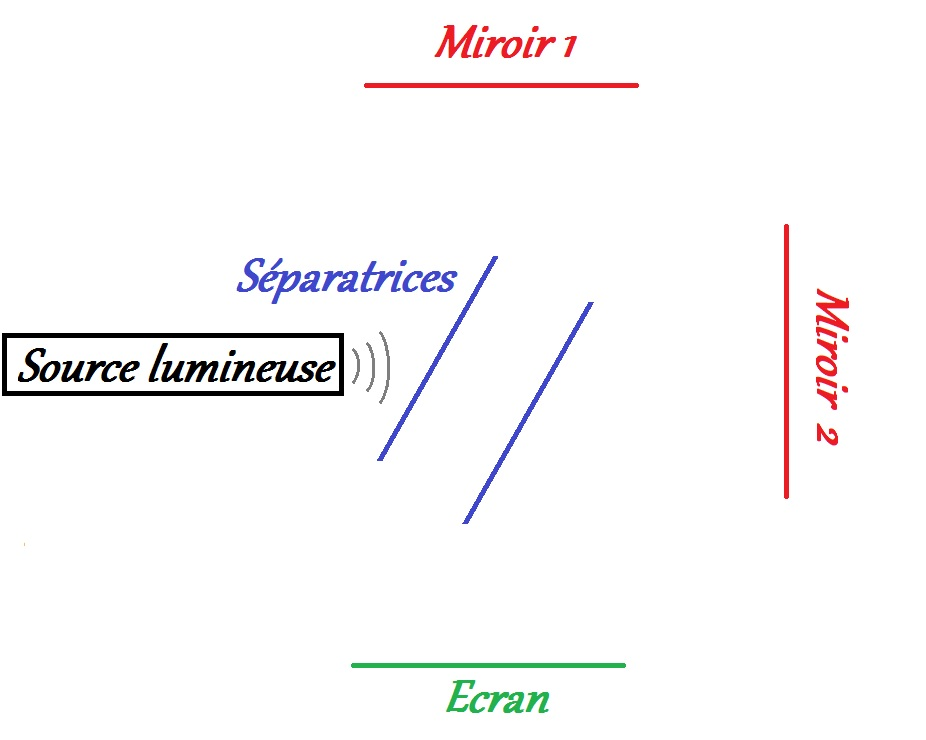
\includegraphics[scale=0.4]{schem1}
	\end{center}
	
	\begin{itemize}[label=$\circ$]
		\item 
		Tout d'abord, il nous a fallu régler le parallélisme de la séparatrice et de la compensatrice. Pour ce faire, nous avons observé les images d'une lunette autocollimatrice à travers les deux lames. Lorsque les images coïncident (i.e se superposent), cela signifie que les deux lames sont parallèles. 
		
		\item 
		Ensuite, il nous a fallu régler la perpendicularité entre les deux miroirs extérieurs un à un. En envoyant un rayon lumineux dans les deux séparatrices, on observe deux taches sur l'écran (voir schéma ci-dessus) qui correspondent chacune à un des miroirs. Le but est de les faire coïncider. 
		
		Pour se faire, on effectue dans un premier temps un réglage à l'œil des miroirs afin de les superposer grossièrement, puis on affine le réglage à la lunette autocollimatrice. Une fois le réglage minutieux de l'un des miroirs fait, on passe au suivant puis on revérifie avec précision la perpendicularité à plusieurs reprises.
	\end{itemize}
	\section{Résultats}
	
	Une fois tous ces réglages effectués (environ 3h), nous pouvons enfin interpréter les résultats. En envoyant un faisceau lumineux d'une lampe de sodium (de couleur jaune orangé), on obtient la figure d'interfranges ci-dessous.
	\begin{center}
		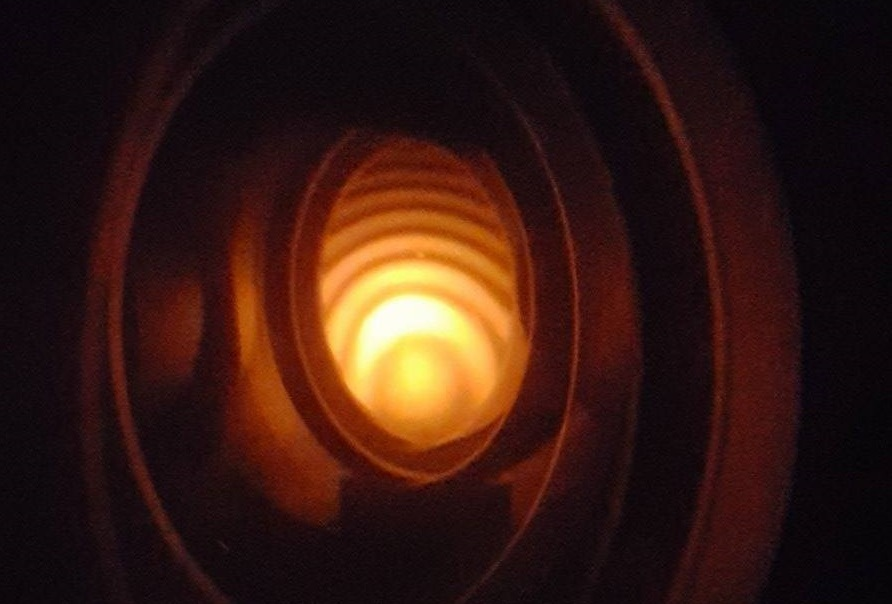
\includegraphics[scale=0.5]{photo1}
		\captionof{figure}{Diffraction vu à travers un filtre pour microscope laser}
	\end{center}
	On peut montrer qu'avec deux longueurs d'onde voisines on trouve un terme de brouillage. En effet, on sait que pour une longueur d'onde donnée on peut approximer l'intensité par :
	$$I_n = I^{0}_{n} (1+\cos(\dfrac{2\pi\delta}{\lambda_n}))$$
	L'intensité de la résultante du doublet de longueurs d'onde $\lambda_1$ et $\lambda_2$ est la somme des intensités. Pour simplifier les calculs, on fait l'hypothèse que :
	\begin{equation}
	I^{0}_{1}=I^{0}_{2}\equiv I_{0}
	\end{equation}
	\begin{align*}
	I &= I_1 + I_2\\
	&= I_0(2+\cos(\dfrac{2\pi\delta}{\lambda_1})+\cos(\dfrac{2\pi\delta}{\lambda_2}))\\
	\end{align*}
	On peut simplifier cette expression en faisant les approximations suivantes : 
	\begin{align}
	\lambda_1+\lambda_2 &\approx 2\lambda_0\\
	\lambda_1\lambda_2 &\approx \lambda_{0}^2\\
	\lambda_2-\lambda_1 &= \Delta\lambda
	\end{align}
	On utilise également la propriété suivante :
	$$\cos(p) + \cos(q) = 2cos(\frac{p+q}{2})cos(\frac{p-q}{2})$$
	D'où
	\begin{align*}
	I &= 2I_0\left\lbrace 1+\cos \left(\frac{\pi  \delta }{\lambda _1}-\frac{\pi  \delta }{\lambda _2}\right) \cos \left(\frac{\pi  \delta }{\lambda _1}+\frac{\pi  \delta }{\lambda _2}\right)\right\rbrace \\
	%
	&= 2I_0\left\lbrace 1+\cos \left(\frac{\pi  \delta  \left(\lambda _1-\lambda _2\right)}{\lambda _1 \lambda _2}\right) \cos \left(\frac{\pi  \delta  \left(\lambda _1+\lambda _2\right)}{\lambda _1 \lambda _2}\right)\right\rbrace\\
	%
	&= 2I_0\left\lbrace 1+\cos \left(\frac{\pi  \delta  \Delta\lambda}{\lambda_{0}^2}\right) \cos \left(\frac{\pi  \delta  2 \lambda_0}{\lambda_{0}^2}\right)\right\rbrace\\
	%
	&= 2I_0\left\lbrace 1+\cos \left(\frac{\pi  \delta  \Delta\lambda}{\lambda_{0}^2}\right) \cos \left(\frac{2 \pi  \delta  }{\lambda_{0}}\right)\right\rbrace
	\end{align*}
	On reconnait un terme d'interférence "classique" : $\cos \left(\frac{2 \pi  \delta  }{\lambda_{0}}\right)$ et un terme de brouillage $\cos \left(\frac{\pi  \delta  \Delta\lambda}{\lambda_{0}^2}\right)$.\\
	Si on considère que $\Delta\lambda<<\lambda_{0}$, le terme de brouillage définit une enveloppe.
	\begin{figure}[h]
		\centering
		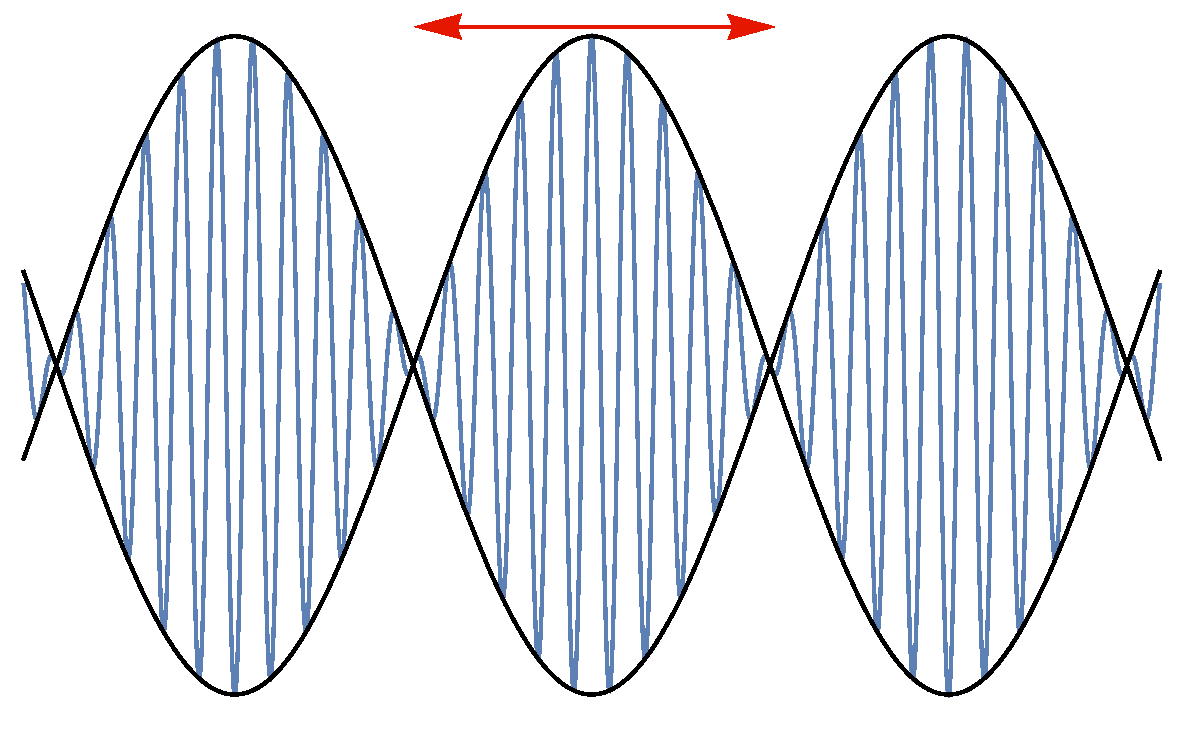
\includegraphics[width=0.5\linewidth]{Brouillage}
		\caption{Comportement du produit des $\cos$}
	\end{figure}
	
	
	Il y a brouillage lorsque :
	
	\begin{alignat*}{3}
	&&\cos \left(\frac{\pi  \delta  \Delta\lambda}{\lambda_{0}^2}\right) & = 0\\
	\iff&& \frac{\pi  \delta  \Delta\lambda}{\lambda_{0}^2} & = \dfrac{\pi}{2} + n\pi\\
	\iff&& \Delta\lambda & = (n+\dfrac{1}{2}) \dfrac{\lambda_{0}^{2}}{\delta}
	\end{alignat*}
	Si on décale un miroir de $\Delta e$, la différence de marche varie de $2\Delta e$ (aller-retour).
	$$\delta = 2\Delta e$$
	
	Ainsi pour deux brouillages consécutifs on a :
	\begin{align*}
	\Delta \lambda  & = \left\lbrace (n+1+\dfrac{1}{2})-(n+\dfrac{1}{2})\right\rbrace \dfrac{\lambda_{0}^{2}}{2\Delta e}\\
	& = \dfrac{\lambda_{0}^{2}}{2\Delta e}
	\end{align*}
	
	On peut alors en mesurant $\Delta e$ entre deux brouillages consécutifs, retrouver une valeur de $\Delta\lambda$. Pour gagner en précision, on peut mesurer plusieurs brouillages et ainsi diminuer l'incertitude sur $\Delta e$
	
	Malheureusement, nous n'avons pas relevé $\Delta e$ correctement pour faire l'application numérique et ainsi retrouver le doublet du sodium.
\end{document}

